%This file will discuss solutions implemented
%This file should be included in doc using \input{file}

\section{Proposed Solutions}

\subsection{Simulations}
For the control design, four separate controllers will be used.  A PID controller will be used to control the altitude of the quad-rotor drone.  Pitch, roll, and yaw will each be controlled respectively by a separate PI controller. These controllers will be first tested and tuned using test inputs.  The physical aspect of the simulation will be defined by a SimScape MultiBody model.  Once this rudimentary model is verified, the simulation will be developed into taking real-time signals from a HID and rendering the flight of the quad-rotor drone in response to user input.

\subsubsection{Simulation Design}
The overall architecture of the proposed design can be seen in Figure \ref{fig:sim_arch}.  The entire system is broken down into six subsystems.  Their specifications are discussed below.  The layout of each subsystem and the overall SimuLink simulation layout may be found in Appendix \ref{appendix:simulink}.

\begin{figure}[H]
	\centering
	\includegraphics[width=0.9\textwidth]{simulation_arch.jpg}
	\label{fig:sim_arch}
	\caption{Proposed Simulation Architecture}
\end{figure}

\begin{enumerate}
	\item \textbf{Input Block:}  This block handles the HID input and pre-configured test signals.  As well as the specifications of limit/scalar values of the input signals.  As the limits will be scalar values, control signal input should be restricted between $-1$ and $1$.
	
	\item \textbf{Feedback Block:}  This block receives the contents specified from the input block as well as the current orientation of the quad-rotor drone in the simulation.  It combines all of these to output an error signal for the pitch, roll, yaw, and altitude controllers.
	
	\item \textbf{Controller Block:}  This block houses the four controllers.  The output of these controllers is normalized to a throttle percentage.
	
	\item \textbf{Pulsewidth Subsystem:}  This block takes the throttle percentage and transform it to a value in microseconds that can be used to define the pulsewidth output of the microcontroller.  Physically, this PWM signal controls the ESCs.
	
	\item \textbf{Motor Characterization:}  This block contains motor thrust data corresponding to characterization tests performed in the first semester.  Functionally this block contains a look up table that relates pulsewidth to thrust and torque for each motor.  The torque value is an approximation based on the value of thrust from the motor.
	
	\item \textbf{Physical Subsystem:}  This block contains the physical subsystem built in SimScape Multibody.  This library allows for the system to be built quickly and easily, as well as providing a (although simple) 3D rendering model.
	
	\item \textbf{3D Rendering:}  This subsystem will handle the real-time rendering of the simulation for flying with input from the HID.
\end{enumerate}

\subsection{Physical Implementation}

The proposed solution incorporates the following components for the physical system architecture.

\begin{itemize}
\item Joystick Controller
\item Base Station Laptop
\item Raspberry Pi 3 Computer
\item Arduino Micro-Controller
\item 10 Degree of Freedom Inertial Measurement Unit
\item Raspberry Pi Camera Module (Future)
\end{itemize}

The system architecture is implemented as depicted in the block diagram shown in Figure \ref{fig:sys_arch}. 

\begin{figure}[H]
	\centering
	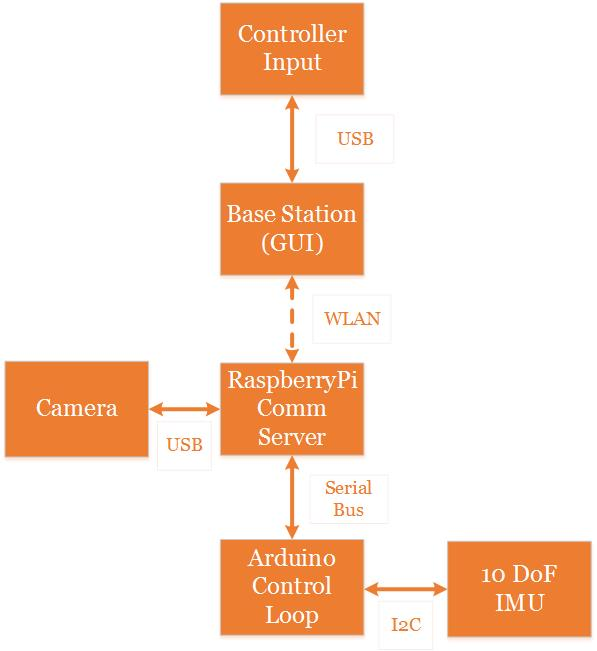
\includegraphics[width=0.7\textwidth]{flowchart-architecture.jpg}
	\caption{System Architecture}
	\label{fig:sys_arch}	
\end{figure}

A joystick controller was used as the control input for its non-spring loaded throttle control. The drone requires an altitude set point from the control input, a spring loaded control input would make the implementation of a constant set point difficult. The base station laptop hosts the GUI and the communication channel software between the USB connected joystick control input and the Raspberry Pi Wi-Fi connection. The Python scripts that enable the communication channels use the sockets library for a server, client Wi-Fi channel and pygame library to acquire control set points from the joystick controller. The inputs from the controller are converted from floats to sets of four bytes for transmission.

The Raspberry Pi is used solely as a communication channel between the base station and the Arduino control loop. The RPi is the server while the base station is considered the client in the connection. The Raspberry Pi relays the received bytes to the Arduino control loop using a serial communication channel. 

The Arduino control loop is used to host the drone function library and main script required for drone flight. The Arduino control loop outline is shown in Figure \ref{fig:ctl_loop}. The gain values for the PID loop is to be determined through simulations. The Arduino initializes all sensors, motors, and communications. The loop then gathers data from the inertial measurement unit and the serial connection to the Raspberry Pi, compares the data and performs a PID loop, finally outputting the results to the ESCs.

\begin{figure}[H]
	\centering
	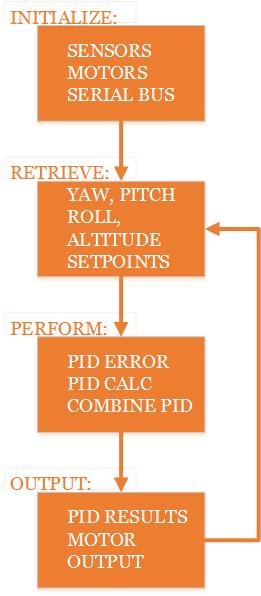
\includegraphics[width=0.7\textwidth]{control-loop.jpg}
	\caption{Arduino Control Loop}
	\label{fig:ctl_loop}	
\end{figure}

Yaw, pitch, roll and altitude are calculated using the accelerometer, gyroscope, magnetometer, barometric pressure sensor and temperature sensor available on the inertial measurement unit. The altitude measurement is completed using the barometric pressure sensor and temperature sensor. The equation to calculate altitude is given as: 

\vspace*{0.2in}
$h=\frac{(\frac{P_{0}}{P})^\frac{1}{5.257}-1)*(T+273.15)}{0.0065}$
\vspace*{0.2in}

$h$ = Difference between Starting Height and Current Height

$P_{0}$ = Initial Pressure at Starting Height

$P$= Current Pressure

$T$ = Current Temperature

The barometric pressure sensor calculation was found to be highly susceptible to noise, several filtering techniques were attempted and a Kalman filter with a feedback comparison is currently in use. This filtering technique is subject to change. All written scripts for the Arduino, Raspberry Pi and the base station communication channel can be found in APPENDIX XXX. 


\subsection{Graphical User Interface}
\subsubsection{Framework Selection}
The basic GUI was to have the ability to call the PS4 controller initialization script and manipulate the axis settings. Because the initialization script was written in Python it was very difficult and time consuming to do this using the C++ version of Qt compared to using PyQt5 where all that had to be done was import the script. Due to each of the scripts that the GUI needs to call are written using Python it was decided to carry on using PyQt5. On top of the ease of importing the scripts using PyQt5 it also allows us to use the vast amount of Python libraries that are available such as matplotlib and pyqtgraph and as discussed, these libraries will be used to plot the sensor data. 

